%!TEX root = ./main.tex
%!TEX encoding = UTF-8 Unicode
\chapter{Task Scheduling and Stack Safety}
\section{Introduction}
\h\ aim to simulate real-time software, this module offers real-time application analysis. This appendix present how to use mechanism that allows to detect task switch and analyze task's stack (usage and corruption).

\noindent Stack Monitoring offers various informations :
\begin{itemize}
	\item \emph{Task Scheduling : }task activation are detected and a T3 trace file could be generated to visualized application behavior in a gantt diagram. The simulator only need task main function symbol and stack size.
	\item \emph{Stack Monitoring and Safety :} provide a good way to evaluate stack use and detect stack failure (like underflow or overflow). The simulator may need some os system function symbol to exclude them from stack failure detection.
\end{itemize}

\emph{Note} : executable file have to be \emph{ELF files}, it's used to resolve function symbol.
% SECTIONS %
\section{Description modification}


Task monitoring only need a slight modification of \h\ processor description. From \h\ view Task monitoring only need to know which instruction or group of instruction is used to CALL, it also uses Stack Pointer value\footnote{SP register have to be defined (for the time being since no generic way to access stack pointer is provided by current \h\ version) SP() is used to get Stack Pointer value.}.

\begin{verbatim} 
 #SP_Check flag should be added to each CALL type instructions (for all views).
\end{verbatim}

\noindent Example on ARM processor description :
\begin{lstlisting}
syntax branch #branch
  "b"
  select
    case #noLink --nothing
    case #withLink  #SP_Check "l"
...

syntax blx #branch #withLink #SP_Check #Thumb 
  "blx"
...

behavior branchInst #branch
    ..
    case #withLink  #SP_Check
	...
	
behavior branchLinkExchangeInst #branch #withLink #Thumb #SP_Check
...

format blx1 #branch #withLink #Thumb #SP_Check -- branch, link and change ISA to Thumb.
...

format blx2 #branch #withLink #Thumb #SP_Check -- branch, link and change ISA to Thumb.
...
 \end{lstlisting}

% SECTIONS %
\section{Compilation flags}
Stack analysis requires significant amount of computation time, so it's an optional tool for \h\ simulator, some building option are required (modification in generated \texttt{Makefile}).

\subsection{Required build options}
Stack monitoring need \emph{action} mechanism (simulation time increase by about 40\%), so the flag \texttt{GADL\_NO\_ACTION} should NOT be defined (see section \ref{sec:cflags}).

\subsection{Task Scheduling}
\noindent Task Scheduling is activated by following building option (simulation time increases about 10\%).
\begin{verbatim}
DEFINES += -DGADL_SP_CHECK_ALLOWED
\end{verbatim}

\subsection{Stack safety monitoring}
\noindent Stack use and safety monitoring is activated by following options (simulation time increase again by about  3\% in worst case).
\begin{verbatim}
DEFINES += -DGADL_SP_FAILURE_CHECK_ALLOWED 
DEFINES += -DGADL_SP_CHECK_ALLOWED
\end{verbatim}

% SECTIONS %
\section{Task Scheduling}
Stack analysis provides to \h\ tools to detect the scheduling of the tasks, in the context of a multi-tasking system. In a multi-tasking system, each task has its own context (stack and register set), it's used to allow detection any user application modification. This tool provides a Gantt from application execution in order to analyze scheduling.

\subsection{Task declaration}
Each Task of application have to be declared to \h\ generated simulator using following function.

\lstset{language=C++}
\begin{lstlisting}
void addTaskToMonitor(string taskName,string functionSym,u32 size);
\end{lstlisting}
\begin{itemize}
	\item  {\tt taskName} is an arbitrary name to describe Task (ex.  {\tt "MainTask"})
	\item  {\tt functionSym} is Task's main function symbol (ex.  {\tt "function\_of\_task1"}).
	\item  {\tt size}  is size of Task's stack (ex.  {\tt 250} a wrong value will result in a simulation failure).
\end{itemize}
\emph{Note:} Two tasks or more can share the same main function, the tool will automatically detect associated stack.

\subsection{Task data}
\noindent Simulator can display list of Task and associated data using following function :
\begin{lstlisting}
void printTaskList()
 \end{lstlisting}
 
 \begin{verbatim}
********************************
* STACK/TASK List Informations *
********************************

Task n 5 (Task 5) : Fct@0 Stack (size=250) : init@0 -1- StackRealUse=0
Task n 4 (Task 4) : Fct@134 Stack (size=250) : init@58d -1- StackRealUse=0
Task n 3 (Task 3) : Fct@122 Stack (size=250) : init@6fa -1- StackRealUse=0
Task n 2 (Task 2) : Fct@110 Stack (size=20) : init@468 -1- StackRealUse=0
Task n 1 (Task 1) : Fct@ee Stack (size=250) : init@368 -1- StackRealUse=0
\end{verbatim}

 \begin{itemize}
	\item  {\tt Task n ..} specific id of task in simulator (0 is {\tt Unkwnon}, then by order of add)
	\item  {\tt task\_name} is task name add by user
	\item  {\tt Fct@...} address of main function of task (automatically detected)
	\item  {\tt size=...} size of stack add by user
	\item  {\tt init@...}  stack initial address
	\item  {\tt -...-} : {\tt 1} if initial value is detected / {\tt 0} if no initial value is detected
	\item  {\tt StaclRealUse=...} not used in this mode
\end{itemize}

\subsection{Task switch data}
\noindent Simulator can display a list of Task switch and activation using following function. Undeclared task events will be associated to task number 0 {\tt  Unkwnon Task}.
\begin{lstlisting}
void printControllerSwitchList();
\end{lstlisting}

\begin{verbatim}
********************************
*       TASK Switch List       *
********************************
Task n 0 --Running   Date=1 SP@0
Task n 5 --Activate  Date=0 SP@0
Task n 5 --Running   Date=0 SP@0
Task n 0 --Running   Date=12784 SP@10fd
Task n 1 --Activate  Date=16316 SP@368
Task n 1 --Running   Date=16316 SP@368
Task n 2 --Activate  Date=20040 SP@468
Task n 2 --Running   Date=20040 SP@468
\end{verbatim}

 \begin{itemize}
	\item  {\tt Task n ..} specific id of task in simulator (0 is {\tt Unkwnon}, then by order of add)
	\item {\tt --.......}  {\tt Running} : stack is in task stack /   {\tt Activate} : task function called
	\item  {\tt Date=...} date in processor cycle (from simulator)
	\item  {\tt SP@... } Stack Pointer value when event occured
\end{itemize}

\subsection{T3 trace generation (Gantt)}
T3\footnote{\url{http://jttrace.rts-software.org} provides a good way to visualize application execution using a Gantt. The simulator can generate a T3} compatible file in order to display a Gantt from application.
\begin{lstlisting}
void writeTraceT3(string path);
\end{lstlisting}
T3 {\tt Idle Task} (maximum ID in T3) is used as {\tt Unknown task} (null ID in \h\ )
\begin{itemize}
	\item  {\tt path} path and name of target file (ex  {\tt "./trace.txt"})
\end{itemize}




% SECTIONS %
\section{Stack Use and Safety Monitoring}
Stack analysis provided tools to find an appropriate stack size by analyzing real stack use of each declared task and detecting failure.

\subsection{Size of stack protection area}
User can choose how much byte upper and lower from the stack area will be associated to failure detection. 
\lstset{language=C++}
\begin{lstlisting}
void setSizeOfStackProtectionArea(type_sp size);
\end{lstlisting}
 \begin{itemize}
	\item  {\tt size} : size of upper and lower protection area used to detect stack failure. TODO dessin!!
\end{itemize}

\subsection{System function exclusion}
Context switch function can be detected as stack failure where there is only a normal behavior of OS, those function can be exclused using following function
\lstset{language=C++}
\begin{lstlisting}
void setExclusionOnSystFunction(string symbol);
\end{lstlisting}
 \begin{itemize}
	\item  {\tt symbol} :  a system function (wich need to be excluded) symbol  (ex  {\tt "tpl\_put\_preempted\_proc"})
\end{itemize}

\subsection{Stack failure message}
Any stack failure detected will automatically be noticed by the simulator providing program adress where it ocured for debugging purpose.

\begin{verbatim}
ERROR in task n 2 (Task 2) @15ac STACK OVERFLOW
ERROR in task n 2 (Task 2) @15ae STACK OVERFLOW
\end{verbatim}

 \begin{itemize}
	\item  {\tt task n ..} : specific id of task in simulator
	\item {\tt taskName} : name of task defined by user
	\item  {\tt @...} : program address where failure occured
	\item  {\tt STACK ...... } : {\tt OVERFLOW} or {\tt UNDERFLOW}
\end{itemize}

\subsection{Stack use print}
\noindent Simulator can display stack's use, using following function :
\begin{lstlisting}
void printTaskList();
 \end{lstlisting}
 
 \begin{verbatim}
********************************
* STACK/TASK List Informations *
********************************

Task n 4 (Task 4) : Fct@134 Stack (size=250) : init@58d -1- StackRealUse=22
Task n 3 (Task 3) : Fct@122 Stack (size=250) : init@6fa -1- StackRealUse=22
Task n 2 (Task 2) : Fct@110 Stack (size=20) : init@468 -1- StackRealUse=19 !! Overflow !!  at PC@15ac
Task n 1 (Task 1) : Fct@ee Stack (size=250) : init@368 -1- StackRealUse=47
\end{verbatim}

 \begin{itemize}
	\item  cf. task scheduling
	\item  {\tt StaclRealUse=...} is the maximum real stack use detected by stack analysis tool
	\item {\tt !! Overflow !! at PC@...} program address of first stack failure
\end{itemize}
 
 % SECTIONS %
\section{Short example of application}
Example included four task, one posses a too small stack to test stack failure dectetion, executable file have to be \emph{ELF files}.
\subsection{Python Script}
Simulator is build with all Stack Analysis options.
\lstset{language=python}
\begin{lstlisting}
#!/usr/bin/python
import sys

# Looks in AT90CAN128 directory to find the processor arch
sys.path.append("./AT90CAN128")
# Provide simulator
from AT90CAN128 import arch	
# Need to access Stack Tools
from AT90CAN128 import stackSpyController

# Create simulator 
f=arch()
# Read executable file (ELF files only)
f.readCodeFile("./AVRTrampolineBinTest1")					

# Get an access to Stack Tools
stackCtrl=f.getStackSpyController()				

# Declaration of Exclusion function for Stack Failure detection
stackCtrl.setExclusionOnSystFunction("tpl_put_preempted_proc");

# Declaration of Tasks in simulator
stackCtrl.addTaskToMonitor("Task 1","startTask_function",250);
stackCtrl.addTaskToMonitor("Task 2","secondTask_function",20);
stackCtrl.addTaskToMonitor("Task 3","thirdTask_function",250);
stackCtrl.addTaskToMonitor("Task 4","fourthTask_function",250);

print "-- task's switching and stack usage analysis --"
f.execInst(10000000) #run until breakpoint

# Print Task data (including real task uses and failure)
print ">> Task List"
stackCtrl.printTaskList();

#Print Task events (activation and switch)
print ">> Switch List"
stackCtrl.printControllerSwitchList()

# Write a T3 file to visualize the Gantt of Task Scheduling
stackCtrl.writeTraceT3("trace.txt");
\end{lstlisting}

\subsection{Result of Simulation}

\begin{verbatim}
$ ./test_stack.py 
-- task's switching and stack usage analysis --
ERROR in task n 2 (Task 2) @15ac STACK OVERFLOW
ERROR in task n 2 (Task 2) @15ae STACK OVERFLOW
>> Task List

********************************
* STACK/TASK List Informations *
********************************

Task n 4 (Task 4) : Fct@134 Stack (size=250) : init@58d -1- StackRealUse=22
Task n 3 (Task 3) : Fct@122 Stack (size=250) : init@6fa -1- StackRealUse=22
Task n 2 (Task 2) : Fct@110 Stack (size=20) : init@468 -1- StackRealUse=19 !! Overflow !!  at PC@15ac
Task n 1 (Task 1) : Fct@ee Stack (size=250) : init@368 -1- StackRealUse=47

>> Switch List

********************************
*       TASK Switch List       *
********************************

Task n 0 --Running   Date=1 SP@0
Task n 1 --Activate  Date=16316 SP@368
Task n 1 --Running   Date=16316 SP@368
Task n 2 --Activate  Date=20040 SP@468
Task n 2 --Running   Date=20040 SP@468
Task n 1 --Running   Date=21222 SP@359
Task n 3 --Activate  Date=25010 SP@6fa
Task n 3 --Running   Date=25010 SP@6fa
Task n 1 --Running   Date=26192 SP@359
Task n 4 --Activate  Date=30012 SP@58d
Task n 4 --Running   Date=30012 SP@58d
Task n 1 --Running   Date=31194 SP@359
\end{verbatim}

\subsection{T3 Gantt from Simulation}

 \begin{itemize}
	\item {\tt  idlle} : is {\tt Unknown task}
	\item  {\tt Task n 0} is the main task (Task 1)
\end{itemize}

 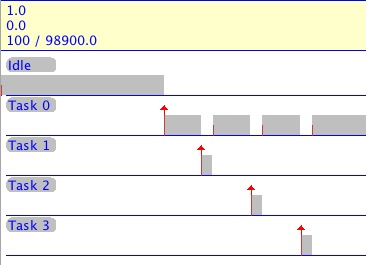
\includegraphics[width=0.8 \linewidth]{../common/images/appendixBSExampleStackAnalysisGantt.jpg}

